%% \documentclass[handout,t]{beamer} % HANDOUT
%% \documentclass[handout,notes=show,t]{beamer} % NOTES
\documentclass[t]{beamer} % SLIDES

\usetheme{SIGIL}
\usepackage{beamer-tools-sigil}

%%
%% some useful macros: mathematical notation etc.
%%

%% abbreviations for logic symbols
\renewcommand{\implies}{\Rightarrow}
\newcommand{\equivalent}{\Leftrightarrow}

%% abbreviations for common number spaces
\newcommand{\setN}[1][]{\mathbb{N}_{#1}} % allows \setN and \setN[0]
\newcommand{\setZ}{\mathbb{Z}}
\newcommand{\setQ}{\mathbb{Q}}
\newcommand{\setR}{\mathbb{R}}

%% sets and (sub-)sets defined by condition
\newcommand{\set}[1]{\{#1\}}
\newcommand{\setdef}[2]{\set{#1\,|\,#2}}
\newcommand{\bigset}[1]{\bigl\{#1\bigr\}}
\newcommand{\bigsetdef}[2]{\bigset{#1\bigm|#2}}
\newcommand{\setscale}[1]{\left\{#1\right\}}
\newcommand{\setdefscale}[2]{\setscale{#1\left|\,#2\right.}}

%% absolute value and norm
\newcommand{\abs}[1]{\lvert #1\rvert}
\newcommand{\bigabs}[1]{\bigl\lvert #1\bigr\rvert}
\newcommand{\absscale}[1]{\left\lvert #1\right\rvert}
\newcommand{\norm}[2][]{\lVert #2\rVert_{#1}}
\newcommand{\bignorm}[2][]{\bigl\lVert #2\bigr\rVert_{#1}}
\newcommand{\normscale}[2][]{\left\lVert #2\right\rVert_{#1}}

%% complement set (with optional index)
\newcommand{\compl}[1][]{\mathcal{C}^{#1}}

%% power set: \powerset{\Sigma^*}
\newcommand{\powerset}[1]{\mathcal{P}(#1)}

%% uparrow: a \ua b = direct dominance in ordered tree
\newcommand{\ua}{\uparrow}

%% left-right arrow: this $\lra$ that
\newcommand{\lra}{\leftrightarrow}

%% expanded engineering notation: 4.2\x\e+5
\newcommand{\e}[2]{10^{\ifthenelse{\equal{#1}{+}}{}{#1}#2}}
\newcommand{\x}{\cdot}

%% arg max & min: \argmax_{x\in C}, \argmin_{x\in C}
\newcommand{\argmax}{\mathop{\text{arg~max}}}
\newcommand{\argmin}{\mathop{\text{arg~min}}}

%% infinitesimal elements: \dx, \dy = \dX{y}, \dz
\newcommand{\dX}[1]{\,\mathit{d{#1}}}
\newcommand{\dx}{\dX{x}}
\newcommand{\dy}{\dX{y}}
\newcommand{\dz}{\dX{z}}

%%% Local Variables: 
%%% mode: latex
%%% TeX-master: ""
%%% End: 
  % basic mathematical notation
%%
%% some useful macros: statistical notation
%%

%% \p{X=k};  \pC{X=k}{Y=l};  \bigp{X_i = k};   \pscale{\frac{Z}{S^2}};
%% probability P(X=k) and conditional probability P(X=k|Y=l), also with larger or scaled parentheses
%% \p[\theta]{X=k};  \pC[\text{interpolated}]{X=k}{Y=l};  ...
%% with optional subscripts (for model probability, null probability, etc.)
\newcommand{\p}[2][]{\mathop{\mathrm{Pr}_{#1}}(#2)}
\newcommand{\pscale}[2][]{\mathop{\mathrm{Pr}_{#1}}\!\left(#2\right)}
\newcommand{\bigp}[2][]{\mathop{\mathrm{Pr}_{#1}}\bigl(#2\bigr)}
\newcommand{\pC}[3][]{\p[#1]{#2\,|\,#3}} 
\newcommand{\pCscale}[3][]{\pscale[#1]{#2\left|\,#3\right.\!}} 
\newcommand{\bigpC}[3][]{\bigp[#1]{#2\!\bigm|\!#3}} 

%% \Exp{X};  \Var{X};  \Exp[0]{X};  \Var[0]{X};  
%% \bigExp{X}; \bigVar{X}; \Expscale{X};  \Varscale{X};
%% expectation E[X] and variance V[X], expectation and variance under null hypothesis, 
%% and variants with largeer or scaled brackets
\newcommand{\Exp}[2][]{\mathrm{E}_{#1}[#2]}
\newcommand{\Var}[2][]{\mathop{\mathrm{Var}}_{#1}[#2]}
\newcommand{\bigExp}[2][]{\mathrm{E}_{#1}\!\bigl[#2\bigr]}
\newcommand{\bigVar}[2][]{\mathop{\mathrm{Var}}_{#1}\bigl[#2\bigr]}
\newcommand{\Expscale}[2][]{\mathrm{E}_{#1}\left[#2\right]}
\newcommand{\Varscale}[2][]{\mathop{\mathrm{Var}}_{#1}\left[#2\right]}

%% \pihat = \hat{\pi}
%% sampling estimate for population probability \pi (may need fine-tuning)
\newcommand{\pihat}{\hat{\pi}}

%% \Entropy{X}, \Entropy{p}, \KL{p}{q}, \MI{X}{Y}
%% \bigEntropy{}, \Entropyscale{}, \bigKL{}{}, \KLscale{}{}, \bigMI{}{}, \MIscale{}{}
%% entropy, KL distance, conditional entropy and mutual information (with scaled variants)
\newcommand{\Entropy}[1]{H[{#1}]}
\newcommand{\bigEntropy}[1]{H\bigl[{#1}\bigr]}
\newcommand{\Entropyscale}[1]{H\left[{#1}\right]}
\newcommand{\KL}[2]{D({#1}\|{#2})}
\newcommand{\bigKL}[2]{D\bigl({#1}\bigm\|{#2}\bigr)}
\newcommand{\KLscale}[2]{D\left({#1}\left\|{#2}\right.\right)}
\newcommand{\MI}[2]{I[{#1};{#2}]}
\newcommand{\bigMI}[2]{I\bigl[{#1};{#2}\bigr]}
\newcommand{\MIscale}[2]{I\left[{#1};{#2}\right]}

%% \corr (correlation) and \cov (covariance) as mathop's
\newcommand{\corr}{\mathop{\mathrm{corr}}}
\newcommand{\cov}{\mathop{\mathrm{cov}}
}
%%% Local Variables: 
%%% mode: latex
%%% TeX-master: ""
%%% End: 
  % notation for probability theory and statistics
%%
%% convenience macros for linear algebra (vectors and matrices)
%%

%% \Vector[i]{x} ... vector variable with optional _superscript_ index in parentheses
%% \Vector[']{x} ... special case: ' superscript not enclosed in parentheses
%% \vx, \vy, \vz ... abbreviations for common vector names
\newcommand{\Vector}[2][]{\mathbf{#2}\ifthenelse{\equal{#1}{}}{}{^{(#1)}}}
\newcommand{\vx}[1][]{\Vector[#1]{x}}
\newcommand{\vy}[1][]{\Vector[#1]{y}}
\newcommand{\vz}[1][]{\Vector[#1]{z}}
\newcommand{\vu}[1][]{\Vector[#1]{u}}
\newcommand{\vv}[1][]{\Vector[#1]{v}}
\newcommand{\vw}[1][]{\Vector[#1]{w}}
\newcommand{\vm}[1][]{\Vector[#1]{m}} 
\newcommand{\va}[1][]{\Vector[#1]{a}} % vectors of coefficients
\newcommand{\vb}[1][]{\Vector[#1]{b}} % for basis
\newcommand{\ve}[1][]{\Vector[#1]{e}} % for standard basis of R^n
\newcommand{\vn}[1][]{\Vector[#1]{n}} % normal vector
\newcommand{\vnull}[1][]{\Vector[#1]{0}} % neutral element

%% \Span{\vb[1],\ldots,\vb[k]} ... span of set of vectors
%% \Rank{...} ... rank of set of vectors or matrix
%% \Det{...}, \det A ... determinant of a set of vectors / a matrix A
%% \Image{f}, \Kernel{f} ... image and kernel of a linear map
\newcommand{\Span}[1]{\mathop{\text{sp}}\left(#1\right)}
\newcommand{\Rank}[1]{\mathop{\text{rank}}\left(#1\right)}
\newcommand{\Det}[1]{\mathop{\text{Det}}\left(#1\right)}
%% \det is already defined in the standard library
\newcommand{\Image}[1]{\mathop{\text{Im}}\left(#1\right)}
\newcommand{\Kernel}[1]{\mathop{\text{Ker}}\left(#1\right)}

%% \dist[2]{\vx}{\vy} ... distance between two vectors (p-metric)
\newcommand{\dist}[3][]{d_{#1}\left(#2, #3\right)}
\newcommand{\bigdist}[3][]{d_{#1}\bigl(#2, #3\bigr)}

%% \sprod{\vu}{\vv} ... scalar product
\newcommand{\sprod}[2]{\left\langle #1, #2 \right\rangle}
\newcommand{\bigsprod}[2]{\bigl\langle #1, #2 \bigr\rangle}


%%% Local Variables: 
%%% mode: latex
%%% TeX-master: ""
%%% End: 
% convenience macros for vectors and matrices

%%%
%%% local configuration adjustments
%%%

%%% You can change pre-defined colours here, override built-in macros from the
%%% style definition and standard library, as well as define macros needed by
%%% all local documents.

%%% e.g. adjust counterpoint (dark green) for data projectors where greens are
%%% far too bright, as well as green component of light colour and pure green
%%% (of course, it's a better solution to adjust the gamma settings of your monitor)
%%
%% \definecolor{counterpoint}{rgb}{.1, .3, 0}
%% \definecolor{light}{rgb}{.45, .3, .55}
%% \definecolor{puregreen}{rgb}{0, .35, 0}

%% ----- extra packages we need to load

\usepackage{tikz}
\usepackage{alltt}              % code examples with nicely formatted comments
\usepackage{rotating}


%% ----- author and copyright messages (so updates are automatically inserted into all files)
\newcommand{\sigilauthors}{%
  \author[SIGIL]{Designed by Stefan Evert\inst{1} and Marco Baroni\inst{2}}
  \institute[Evert \& Baroni]{
    \inst{1}Computational Corpus Linguistics Group\\
    Friedrich-Alexander-Universit�t Erlangen-N�rnberg, Germany
    \and
    \inst{2}Center for Mind/Brain Sciences (CIMeC)\\
    University of Trento, Italy
  }
}
\newcommand{\sigilcopyright}{%
  \date[sigil.r-forge.r-project.org]{%
    \primary{\footnotesize\url{http://SIGIL.r-forge.r-project.org/}}\\
    \light{\tiny Copyright \textcopyright\ 2007--2018 Evert \& Baroni}}
}

%% ----- automatically show TOC reminder at beginning of each subsection
\AtBeginSubsection[]
{
  \begin{frame}
    \frametitle{Outline}
    \tableofcontents[current,currentsubsection]
  \end{frame}
}

%% ----- some useful macros for the SIGIL course

\newenvironment{Rcode}[1][]{%
  \setbeamercolor{block title}{fg=counterpoint,bg=counterpoint!15!white}%
  \setbeamercolor{block body}{bg=counterpoint!5!white}\small%
  \begin{block}{#1}\begin{alltt}\ungap[1]}{%
      \ungap[1]\end{alltt}\end{block}} % \end{alltt} ... to deconfuse emacs

%% use \sbox{\Rbox} ... \usebox{\Rbox} to insert arbitray latex into Rcode environment
\newsavebox{\Rbox}

%% > plot(x,y)      \REM{this produces a scatterplot}
\newcommand{\REM}[2][\small]{\textsf{#1\color{primary}\# #2}}

%% nice colour for R output: \begin{Rout} .. \end{Rout}
\newenvironment{Rout}[1][\footnotesize]{%
  \begin{footnotesize}#1\color{secondary}\bfseries}{%
    \color{black}\mdseries\end{footnotesize}}

%% rotated column labels for table (to fit long text into narrow columns
\newcommand{\rotLabel}[2][60]{\begin{rotate}{#1}#2\end{rotate}}
 % local adjustments to configuration and macros

%%%%%%%%%%%%%%%%%%%%%%%%%%%%%%%%%%%%%%%%%%%%%%%%%%%%%%%%%%%%%%%%%%%%%%
%% Titlepage

\title[4a.\ Collocations (part 1)]{Unit 4: Collocations \& Contingency
  Tables (Pt.~1)}
\subtitle{Statistics for Linguists with R -- A SIGIL Course}
\sigilauthors
\sigilcopyright

\begin{document}

\frame{\titlepage}

%%%%%%%%%%%%%%%%%%%%%%%%%%%%%%%%%%%%%%%%%%%%%%%%%%%%%%%%%%%%%%%%%%%%%%

\section*{Outline}
\frame{ 
  \frametitle{Outline}
  \tableofcontents
}

%%%%%%%%%%%%%%%%%%%%%%%%%%%%%%%%%%%%%%%%%%%%%%%%%%%%%%%%%%%%%%%%%%%%%%%%
\section{Collocations \& multiword expressions (MWE)}

\newcommand{\tc}[1]{\textcite{\large #1}}
\begin{frame}
  \frametitle{What is a collocation?}

  \begin{itemize}
  \item Words tend to appear in typical, recurrent combinations:
    \begin{tabbing}
      $\quad$ \tc{day} \=and \tc{night} \\
      \> \tc{ring} \=and \tc{bell} \\
      \>\> \tc{milk} \=and \tc{cow} \\
      \>\>\> \tc{kick} \=and \tc{bucket} \\
      \>\>\>\> \tc{brush} and \tc{teeth}
    \end{tabbing}
  \item[] \pause
  \item[] \hand\ such pairs are called \h{collocations} (Firth 1957)
    \begin{itemize}
    \item the meaning of a word is in part determined by its characteristic
      collocations
    \item \emph{``You shall know a word by the company it keeps!''}
    \end{itemize}
  \end{itemize}
\end{frame}

\begin{frame}
  \frametitle{What is a collocation?}

  \begin{itemize}
  \item Native speakers have strong \& widely shared intuitions\\
    about such habitual word combinations
  \item[]
  \item Collocational knowledge is essential for non-native speakers in order
    to sound natural \so ``idiomatic English'' 
  \end{itemize}
\end{frame}

\begin{frame}
  \frametitle{An important distinction \ldots}
  \framesubtitle{\ldots\ which has been the cause of many misunderstandings.}

  \begin{itemize}
  \item \h{Collocations} are an empirical linguistic phenomenon
    \begin{itemize}
    \item can be observed in corpora \& quantified
    \item provide a window to lexical meaning and word usage
    \item applications in language description (Firth 1957) and computational
      lexicography (Sinclair 1966, 1991) 
    \item[]\pause
   \end{itemize}
  \item In contrast to lexicalised \h{multiword expressions}
    \begin{itemize}
    \item MWE need to be lexicalised (i.e., stored as units) because of
      certain idiosyncratic properties
    \item non-compositionality, non-substitutability, non-modifiability
      (Manning \& Sch�tze 1999)
    \item MWE are not directly observable, defined by linguistic tests (e.g.\
      substitution test) and native speaker intuitions
    \item[]\pause
    \end{itemize}
  \item[\hand] but the term ``collocations'' has been used for both concepts
  \end{itemize}
\end{frame}

%%%%%%%%%%%%%%%%%%%%%%%%%%%%%%%%%%%%%%%%%%
\subsection{What are collocations?}

\begin{frame}
  \frametitle{But what \emph{are} collocations?}

  \begin{itemize}
  \item Empirically, collocations are words that show an \h{attraction}
    towards each other (or a ``mutual expectancy'')
    \begin{itemize}
    \item in other words, a tendency to occur near each other
    \item collocations can also be understood as statistically salient
      patterns that can be exploited by language learners 
    \end{itemize}
  \item[]\pause
  \item Linguistically, collocations are an \h{epiphenomenon} \ldots\\\pause
    $\qquad$ \ldots\ some might also say a hotchpotch \ldots\\\pause
    \ldots\ of many different linguistic causes that lie behind the observed
    surface attraction.
  \end{itemize}
\end{frame}

\begin{frame}
  \frametitle{Collocates of \emph{bucket} (n.)}
  
  \ungap
  \begin{center}
    \begin{scriptsize}
      \begin{tabular}{>{\itshape}lr}
        \toprule
        \textup{noun} & $f$ \\
        \midrule
      water & 183 \\
      spade &  31 \\
    plastic &  36 \\
       slop &  14 \\
       size &  41 \\
        mop &  16 \\
     record &  38 \\
     bucket &  18 \\
        ice &  22 \\
       seat &  20 \\
       coal &  16 \\
    density &  11 \\
    brigade &  10 \\
  algorithm &   9 \\
     shovel &   7 \\
  container &  10 \\
       oats &   7 \\
       sand &  12 \\
      Rhino &   7 \\
  champagne &  10 \\
        \bottomrule
      \end{tabular}
      \hspace{5mm}
      \begin{tabular}{>{\itshape}lr}
        \toprule
        \textup{verb} & $f$ \\
        \midrule
      throw & 36 \\
       fill & 29 \\
  randomize &  9 \\
      empty & 14 \\
        tip & 10 \\
       kick & 12 \\
       hold & 31 \\
      carry & 26 \\
        put & 36 \\
      chuck &  7 \\
       weep &  7 \\
       pour &  9 \\
      douse &  4 \\
      fetch &  7 \\
      store &  7 \\
       drop &  9 \\
       pick & 11 \\
        use & 31 \\
       tire &  3 \\
      rinse &  3 \\
        \bottomrule
      \end{tabular}
      \hspace{5mm}
      \begin{tabular}{>{\itshape}lr}
        \toprule
        \textup{adjective} & $f$ \\
        \midrule
          large & 37 \\
  single-record &  5 \\
           cold & 13 \\
     galvanized &  4 \\
     ten-record &  3 \\
           full & 20 \\
          empty &  9 \\
       steaming &  4 \\
     full-track &  2 \\
   multi-record &  2 \\
          small & 21 \\
          leaky &  3 \\
     bottomless &  3 \\
     galvanised &  3 \\
           iced &  3 \\
          clean &  7 \\
         wooden &  6 \\
            old & 19 \\
       ice-cold &  2 \\
     anti-sweat &  1 \\
        \bottomrule
      \end{tabular}
    \end{scriptsize}
  \end{center}
\end{frame}

\begin{frame}
  \frametitle{Collocates of \emph{bucket} (n.)}

  \begin{itemize}
  \item opaque \h{idioms} (\emph{kick the bucket}, but often used literally)
  \item \h{proper names} (\emph{Rhino Bucket}, a hard rock band)
  \item noun \h{compounds}, lexicalised or productively formed\\
    (\emph{bucket shop}, \emph{bucket seat}, \emph{slop bucket}, \emph{champagne bucket})
  \item \h{lexical collocations} = semi-compositional combinations\\
    (\emph{weep buckets}, \emph{brush one's teeth}, \emph{give a speech})
  \item cultural \h{stereotypes} (\emph{bucket and spade})
  \item \h{semantic compatibility} (\emph{full, empty, leaky bucket};\\
    \emph{throw, carry, fill, empty, kick, tip, take, fetch a bucket})
  \item \h{semantic fields} (\emph{shovel, mop}; hypernym \emph{container})
  \item \h{facts} of life (\emph{wooden bucket}; \emph{bucket of water, sand, ice, \ldots})
  \item often sense-specific (\emph{bucket size}, \emph{randomize to a bucket})
    
  \end{itemize}
\end{frame}

\begin{frame}
  \frametitle{Operationalising collocations}

  \begin{itemize}
  \item Firth introduced collocations as an essential component of his
    methodology, but without any clear definition
    \begin{itemize}
    \item[] \textcite{Moreover, these and other technical words are given
        their `meaning' by the restricted language of the theory, and by
        applications of the theory in quoted works. \textup{(Firth 1957,
          169)}}
    \end{itemize}
  \item[]
  \item Empirical concept needs to be formalised and quantified
    \begin{itemize}
    \item intuition: collocates are ``attracted'' to each other, i.e.\
      they tend to occur near each other in text%
      \pause
    \item definition of ``nearness'' \so \h{cooccurrence}%
      \pause
    \item quantify the strength of attraction between collocates based on
      their recurrence \so cooccurrence \h{frequency}
    \end{itemize}
  \item[]\pause
  \item[\hand] We will consider word pairs $(w_1,w_2)$ such as (\emph{brush},
    \emph{teeth})
  \end{itemize}
\end{frame}

%%%%%%%%%%%%%%%%%%%%%%%%%%%%%%%%%%%%%%%%%%
\subsection{Types of cooccurrence}

\begin{frame}
  \frametitle{Different types of cooccurrence}

  \begin{enumerate}
  \item \h{Surface cooccurrence}
    \begin{itemize}
    \item criterion: surface distance measured in word tokens
    \item words in a \emph{collocational span} around the node word,\\
      may be symmetric (L5, R5) or asymmetric (L2, R0)
    \item traditional approach in lexicography and corpus linguistics
    \end{itemize}
  \item[]\pause
  \item \h{Textual cooccurrence}
    \begin{itemize}
    \item words cooccur if they are in the same text segment\\
      (sentence, paragraph, document, Web page, \ldots)
    \item often used in Web-based research (\so Web as corpus)
    \end{itemize}
  \item[]\pause
  \item \h{Syntactic cooccurrence}
    \begin{itemize}
    \item words in a specific syntactic relation, e.g.
      \begin{itemize}
      \item adjective modifying noun
      \item subject / object noun of verb
      \item N \emph{of} N and similar patterns
      \end{itemize}
    \item suitable for extraction of MWE (Krenn \& Evert 2001)
    \end{itemize}
  \end{enumerate}
\end{frame}
  
\begin{frame}
  \frametitle{Types of cooccurrence: examples}
  \framesubtitle{Surface cooccurrence}

  \begin{itemize}
  \item \h{Surface cooccurrences} of $w_1$ = \emph{hat} with $w_2$ = \emph{roll}
    \begin{itemize}
    \item symmetric \underline{window} of four words (L4, R4)
    \item limited by sentence boundaries
    \end{itemize}
  \end{itemize}

  \begin{center}
    \colorbox{blue!20!white}{%
      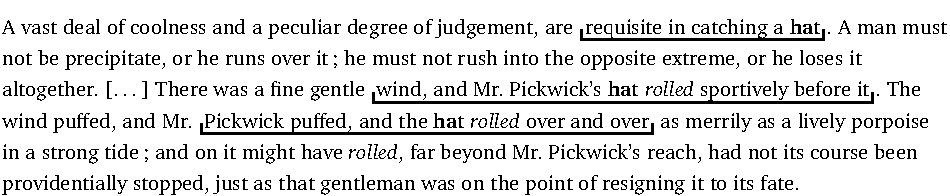
\includegraphics[width=\textwidth,height=3cm]{img/cooc_distance}}
  \end{center}

  \pause
  \begin{itemize}
  \item \h{coocurrence frequency} $f = 2$
  \item \h{marginal frequencies} $f_1 = f_2 = 3$
  \end{itemize}
\end{frame}

\begin{frame}
  \frametitle{Types of cooccurrence: examples}
  \framesubtitle{Textual cooccurrence}

  \begin{itemize}
  \item \h{Textual cooccurrences} of $w_1$ = \emph{hat} and $w_2$ = \emph{over}
    \begin{itemize}
    \item textual units = sentences
    \item multiple occurrences within a sentence ignored
    \end{itemize}
  \end{itemize}

  \begin{center}
    \colorbox{blue!20!white}{%
      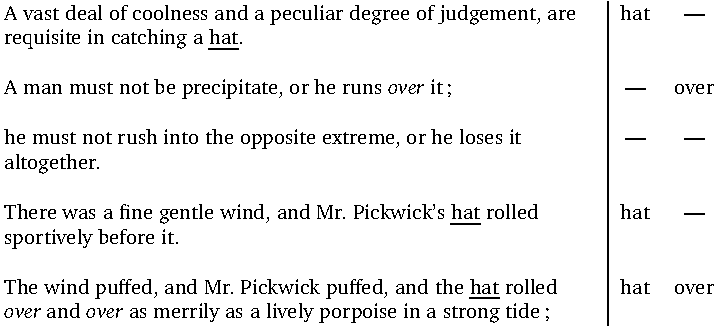
\includegraphics[scale=.7]{img/cooc_sentence}}
  \end{center}

  \pause
  \begin{itemize}
  \item coocurrence frequency $f = 1$
  \item marginal frequencies $f_1 = 3$,  $f_2 = 2$
  \end{itemize}
\end{frame}

\begin{frame}
  \frametitle{Types of cooccurrence: examples}
  \framesubtitle{Syntactic cooccurrence}

  \begin{itemize}
  \item \h{Syntactic cooccurrences} of adjectives and nouns
    \begin{itemize}
    \item every instance of the syntactic relation of interest is\\ extracted
      as a \h{pair token}
    \end{itemize}
  \end{itemize}

  \begin{center}
    \colorbox{blue!20!white}{%
      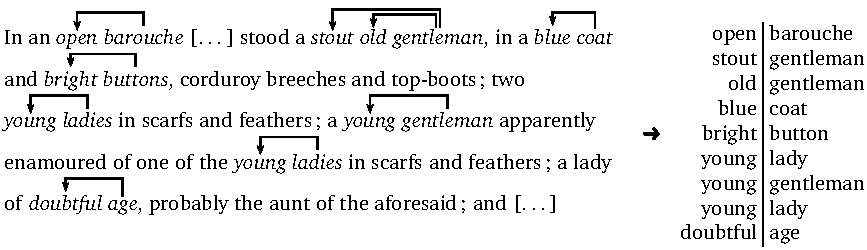
\includegraphics[scale=.7]{img/cooc_syntactic}}
  \end{center}

  \pause
  Cooccurrency frequency data for \emph{young gentleman}:
  \begin{itemize}
  \item coocurrence frequency $f = 1$
  \item marginal frequencies $f_1 = f_2 = 3$
  \end{itemize}
\end{frame}

%%%%%%%%%%%%%%%%%%%%%%%%%%%%%%%%%%%%%%%%%%%%%%%%%%%%%%%%%%%%%%%%%%%%%%%%
\section{Quantifying the attraction between words}

\begin{frame}
  \frametitle{Quantifying attraction}

  \begin{itemize}
  \item Quantitative measure for attraction between words based on their
    recurrence \so \h{cooccurrence frequency}%
    \pause
  \item But cooccurrence frequency is not sufficient
    \begin{itemize}
    \item bigram \emph{is to} occurs $f=$ 260 times in Brown corpus
    \item but both components are so frequent ($f_1\approx $ 10,000 and\\
      $f_2\approx $ 26,000) that one would also find the bigram 260 times if
      words in the text were arranged in completely random order
    \end{itemize}
    \pause%
    \hand\ take \h{expected frequency} into account as ``baseline''
  \item Statistical model required to bring in notion of ``chance
    cooccurrence'' and to adjust for sampling variation
  \item[]\pause 
    \begin{itemize}
    \item[\hand] NB: bigrams can be understood either as syntactic (adjacency
      relation) or as surface cooccurrences (L1, R0 or L0, R1)
    \end{itemize}
  \end{itemize}
\end{frame}

\begin{frame}
  \frametitle{Attraction as statistical association}
  
  \begin{itemize}
  \item Tendency of events to cooccur = \h{statistical association}
    \begin{itemize}
    \item statistical measures of association computed on\\ \h{contingency
        tables}, resulting from a \h{cross-classification}\\ of a set of
      ``items'' according to two (binary) factors
    \item cross-classifying factors represent the two events
    \end{itemize}
  \item[]\pause
  \item Application to word cooccurrence data
    \begin{itemize}
    \item most natural for \h{syntactic cooccurrences}
    \item ``items'' are pair tokens = instances of syntactic relation
    \item factor 1: Is first component of pair token an instance of word type
      $w_1$?
    \item factor 2: Is second component of pair token an instance of word type
      $w_2$?
    \end{itemize}
  \end{itemize}
\end{frame}

%%%%%%%%%%%%%%%%%%%%%%%%%%%%%%%%%%%%%%%%%%
\subsection{Contingency tables}

\begin{frame}
  \frametitle{Contingency table of observed frequencies}
  \framesubtitle{For \h{syntactic} cooccurrences}

  \centering

  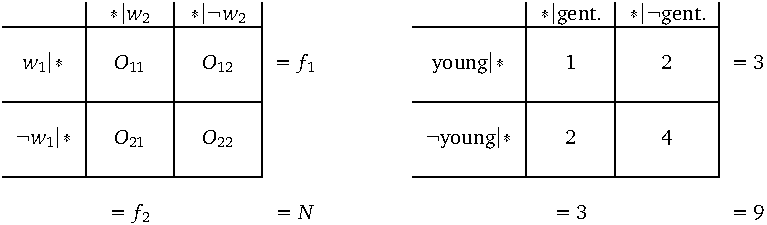
\includegraphics[width=\textwidth]{img/cont_table_syntactic}

  \vspace{1cm}
  \colorbox{blue!20!white}{%
    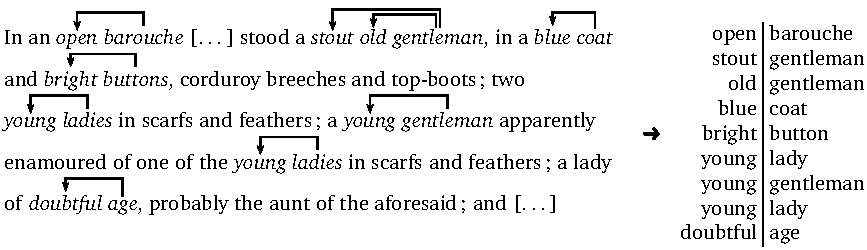
\includegraphics[scale=.6]{img/cooc_syntactic}}

\end{frame}

\begin{frame}
  \frametitle{Contingency table of observed frequencies}
  \framesubtitle{For \h{textual} cooccurrences (sentence windows)}

  \centering

  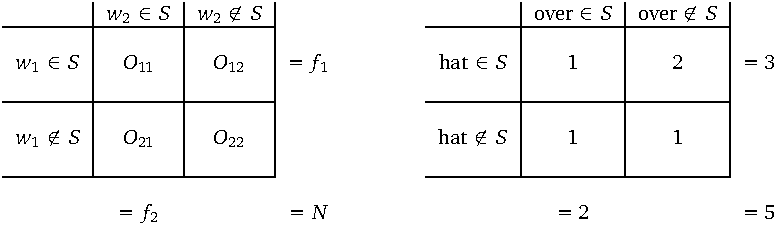
\includegraphics[width=\textwidth]{img/cont_table_sentence}

  \vspace{5mm}
  \colorbox{blue!20!white}{%
    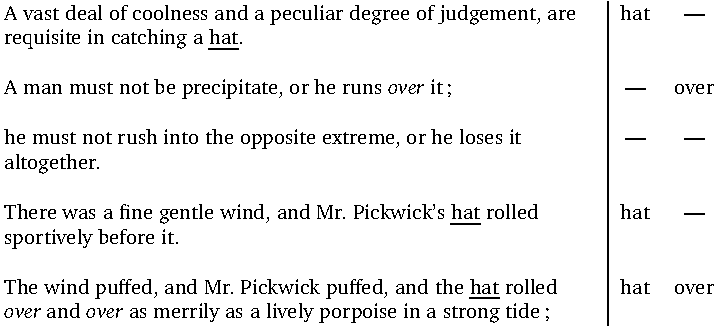
\includegraphics[scale=.6]{img/cooc_sentence}}

\end{frame}

\begin{frame}
  \frametitle{Contingency table of observed frequencies}
  \framesubtitle{For \h{surface} cooccurrences (L4, R4)}

  \centering

  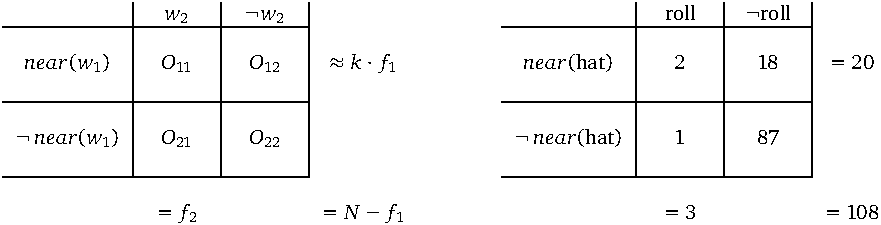
\includegraphics[width=\textwidth]{img/cont_table_distance}

  \vspace{5mm}
  \colorbox{blue!20!white}{%
    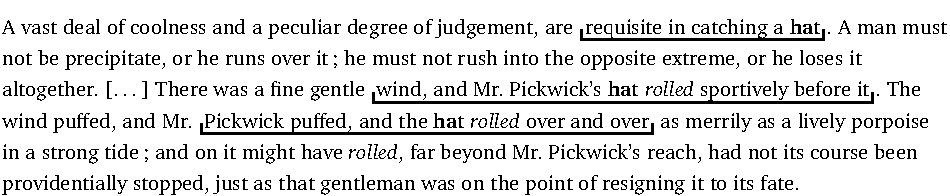
\includegraphics[scale=.6]{img/cooc_distance}}

  \vspace{5mm}
  \begin{footnotesize}
    \parbox{11cm}{%
      \h{More details:} Section 5.1 of Evert, Stefan
      (2008). \secondary{Corpora and collocations.}  In A.~L{\"u}deling and
      M.~Kyt{\"o} (eds.), {\em Corpus Linguistics.  An International
        Handbook}, article~58. Mouton de Gruyter, Berlin.%
    }
  \end{footnotesize}

\end{frame}

\begin{frame}
  \frametitle{Measuring association in contingency tables}

  \begin{itemize}
  \item[A)] Measures of \h{significance}
    \begin{itemize}
    \item apply statistical hypothesis test with null hypothesis $H_0$:
      independence of rows and columns
    \item $H_0$ implies there is no association between $w_1$ and $w_2$
    \item \h{association score} = test statistic or p-value
    \item one-sided vs.\ two-sided tests
    \end{itemize}
    \hand\ amount of evidence for association between $w_1$ and $w_2$
  \item[]\pause
  \item[B)] Measures of \h{effect-size}
    \begin{itemize}
    \item compare observed frequencies $O_{ij}$ to \h{expected frequencies}
      $E_{ij}$ under $H_0$ (\so later)
    \item or estimate conditional prob.\ $\pC{w_2}{w_1}$, $\pC{w_1}{w_2}$,
      etc.
    \item maximum-likelihood estimates or confidence intervals
    \end{itemize}
    \hand\ strength of the attraction between $w_1$ and $w_2$
  \end{itemize}
\end{frame}

%%%%%%%%%%%%%%%%%%%%%%%%%%%%%%%%%%%%%%%%%%
\subsection{Contingency tables and hypothesis tests in R}

\begin{frame}[fragile]
  \frametitle{Contingency tables in R}

  \begin{itemize}
  \item Contingency table is represented as a \h{matrix} in R,\\
    i.e.\ a rectangular array of numbers
    \begin{itemize}
    \item looks like numeric data frame, but different internally
    \end{itemize}
  \item E.g.\ for the following observed frequencies:\\
    $O_{11} = 10$, $O_{12} = 47$, $O_{21} = 82$, $O_{22} = 956$
  \end{itemize}
  \pause

  \begin{alltt}
> A <- matrix(c(10,47,82,956), nrow=2, ncol=2, byrow=TRUE)
> A

\REM{construct matrix from row (or column) vectors}
> A <- rbind(c(10,47), c(82,956))
  \end{alltt}
\end{frame}

\begin{frame}[fragile]
  \frametitle{Independence tests in R}

  \begin{alltt}
\REM{chi-squared test is the standard independence test}
> chisq.test(A)

\REM{use test statistic as association score, p-value for interpretation}

\REM{Is there significant evidence for a collocation?}

\REM{Fisher's exact test works better for small samples and skewed tables}
> fisher.test(A)
  \end{alltt}
\end{frame}

\begin{frame}
  \frametitle{Interpreting hypothesis tests as association scores}

  \begin{itemize}
  \item Establishing significance
    \begin{itemize}
    \item p-value = total probability of observed contingency table and all
      more ``extreme'' tables if $H_0$ is true
    \item theory: $H_0$ can be rejected if p-value is below accepted
      \h{significance level} (commonly $.05$, $.01$ or $.001$)
    \item practice: nearly all word pairs are highly significant
    \end{itemize}
    \pause
  \item Test statistic = significance association score
    \begin{itemize}
    \item \h{convention} for association scores: high scores indicate strong
      attraction between words
    \item satisfied by \h{test statistic} $X^2$, but not by p-value
    \item Fisher's test: transform p-value, e.g.\ $-\log_{10} p$
    \end{itemize}
    \pause
  \item Odds ratio as measure of effect size
    \begin{itemize}
    \item Fisher's test also provides estimate for \h{odds ratio} $\theta$, an
      effect-size measure for association strength
    \item log odds ratio $\log \theta$ as effect-size association score\\
      (0 for independence, large values indicate strong attraction)
    \item conservative estimate = lower bound of confidence interval 
    \end{itemize}
  \end{itemize}
\end{frame}

\begin{frame}[fragile]
  \frametitle{Association scores from hypothesis tests}

  \begin{alltt}
\REM{chi-squared statistic \(X^2\) as association score}
> chisq.test(A)\$statistic

\REM{p-value of Fisher's test and corresponding association score}
> fisher.test(A)\$p.value
> -log10(fisher.test(A)\$p.value)

\REM{NB: chi-squared and Fisher scores are not on same scale}

\REM{log odds ratio and conservative estimate}
> log(fisher.test(A)\$estimate)
> log(fisher.test(A)\$conf.int[1])

> str(fisher.test(A))  \REM{or read help page carefully}
  \end{alltt}
\end{frame}

\begin{frame}[fragile]
  \frametitle{Association scores from hypothesis tests}

  \begin{alltt}
\REM{define two further (invented) contingency tables}
> B1 <- rbind(c(16,84), c(84,816))
> B2 <- rbind(c(1,99), c(99,801))

\REM{calculate chi-squared and Fisher scores for the two tables,}
\REM{as well as estimates for their log odds ratios}

\REM{Do the results look plausible to you? What is wrong?}
  \end{alltt}
\end{frame}

\begin{frame}[fragile]
  \frametitle{One-sided vs.\ two-sided association scores}

  \begin{itemize}
  \item Chi-squared and Fisher are \h{two-sided} tests
    \begin{itemize}
    \item calculate high association scores (= low p-values) both for strong
      positive association (\h{attraction}) and for strong negative
      association (\h{repulsion})
    \item we are usually interested in attraction only (unless we are looking
      for ``anti-collocations'')
    \end{itemize}
    \pause
  \item Fisher can be applied as \h{one-sided} test
    \begin{itemize}
    \item we are only interested in the \h{alternative} to $H_0$ that there is
      greater than chance cooccurrence, not in the alternative of less than
      chance cooccurrence
    \end{itemize}
  \end{itemize}
  
  \begin{alltt}
> fisher.test(B1, alternative="greater")    
\REM{high scores (significance and log odds ratio)}
> fisher.test(B2, alternative="greater")    
\REM{low scores (significance and log odds ratio)}
  \end{alltt}
\end{frame}

%%%%%%%%%%%%%%%%%%%%%%%%%%%%%%%%%%%%%%%%%%
\subsection{Practice session}

\begin{frame}
  \frametitle{Practice: bigrams in the Brown corpus}

  \begin{itemize}
  \item Data set of bigrams with $f\geq 5$ in the Brown corpus
    \begin{itemize}
    \item included in \texttt{SIGIL} package as \texttt{BrownBigrams}
    \item available on course homepage as \texttt{brown\_bigrams.tbl}
    \end{itemize}
  \item[]
  \item 24,167 rows (= bigrams) with variables:
    \begin{itemize}
    \item \h{id} = numeric ID of bigram
    \item \h{word1} = first word (e.g.\ \emph{long} for \emph{long time})
    \item \h{pos1} = part-of-speech code (e.g.\ \texttt{J} for adjective)
    \item \h{word2} = second word (e.g.\ \emph{time} for \emph{long time})
    \item \h{pos2} = part-of-speech code (e.g.\ \texttt{N} for noun)
    \item \h{O11} = observed cooccurrence frequency $O_{11}$
    \item \h{O12} = observed frequency $O_{12}$
    \item \h{O21} = observed frequency $O_{21}$
    \item \h{O22} = observed frequency $O_{22}$
    \end{itemize}
  \end{itemize}
\end{frame}

\begin{frame}[fragile]
  \frametitle{Practice: bigrams in the Brown corpus}

  \begin{alltt}
> library(SIGIL)
> Brown <- BrownBigrams

\REM{Now select a number of bigrams (e.g. low and high cooccurrence}
\REM{frequency, or specific part-of-speech combinations), construct}
\REM{the corresponding contingency tables in \texttt{matrix} form,}
\REM{and calculate the different association scores you know.}
\REM{Can you find a bigram with strong negative association?}

\REM{NB: These are the same tests that we have used for corpus frequency}
\REM{comparisons. Assume that a certain expression occurs 50 times in the}
\REM{100,000 tokens of corpus A, and twice in the 1,000 tokens of corpus B.}
\REM{What is an appropriate contingency table for these data, and what}
\REM{results do you obtain from the chi-squared and Fisher test?}
  \end{alltt}
\end{frame}

%%%%%%%%%%%%%%%%%%%%%%%%%%%%%%%%%%%%%%%%%%%%%%%%%%%%%%%%%%%%%%%%%%%%%%
%% References (if any)

%% \frame[allowframebreaks]{
%%   \frametitle{References}
%%   \bibliographystyle{natbib-stefan}
%%   \begin{scriptsize}
%%     \bibliography{sigil}
%%   \end{scriptsize}
%% }

\end{document}
